\section{Positive Control: Nonlinear Readouts Also Produce Flat Curves}
\label{sec:pc}

Proposition~\ref{prop:jac} gives a sufficient condition for a
readout's Jacobian with respect to $\Z$ to be constant. The natural
prediction is that a readout violating this condition --- a readout
\emph{nonlinear} in $\Z$ --- should produce a non-flat rank-$k$
curve. This section runs that positive control. The hypothesis --- that
readout linearity is the full mechanism --- is falsified.

\subsection{Four readout variants}

We constructed four readout variants, replacing only
$\phi:\R^{d\times d}\to\R^D$ in the matrix bottleneck and leaving
all other training hyperparameters fixed (gpt2-small, ProsQA,
$\gamma=0$, six latent positions, $d=16$, 25 epochs, batch 16, seed
$1337$, AdamW at $\text{lr}=10^{-4}$). Note that all four positive
controls are trained at $\gamma=0$ --- that is, without the CODI
L1-at-colon distillation term. The flat rank-$k$ curves therefore hold
for the cross-entropy loss through the matrix bottleneck alone, not for
the CODI distillation loss specifically. The variants are:

\begin{description}
\setlength\itemsep{3pt}
\item[Bilinear.] $\phi(\Z) = W\,\operatorname{probes}(\Z)$ where
      $\operatorname{probes}(\Z)_k = u_k^\top \Z v_k$ for $K=d^2$
      learned probe pairs $(u_k,v_k)\in\R^d\times\R^d$. Each probe
      is a Frobenius inner product $\langle u_k v_k^\top,
      \Z\rangle_F$, which is linear in $\Z$. This variant is a
      reparametrization control --- it verifies that the low-rank
      factoring of $W_{\text{down}}$ does not change the curve.
\item[Bilinear+GELU.] $\phi(\Z) = W\,\operatorname{GELU}(
      \operatorname{probes}(\Z))$. The GELU gates each probe's
      contribution by a scalar that depends on $\Z$, making $\phi$
      nonlinear in $\Z$. The Jacobian is not constant, but its column
      space in $\R^{d\times d}$ is fixed (the span of the
      $u_k v_k^\top$); only column magnitudes vary with $\Z$. This is
      a relatively mild violation of Proposition~\ref{prop:jac};
      SVD-augmented (below) tests a stronger violation in which the
      Jacobian's column space depends on $\Z$'s singular structure.
\item[SVD-augmented.] $\phi(\Z) = W_{\text{down}}\vecop(\Z) +
      \operatorname{MLP}(\sigma(\Z))$, where $\sigma(\Z)\in\R^d$ is
      the vector of singular values. The MLP feeds the $d=16$
      singular values through two dense layers with GELU. We compute
      $\sigma(\Z)$ via \texttt{torch.linalg.svdvals}, whose backward
      is documented as unconditionally numerically stable (in contrast
      to full \texttt{torch.linalg.svd}, whose backward is unstable
      at near-coincident singular values). This variant explicitly
      exposes rank to the optimizer. Empirically, SVD-augmented's
      best accuracy ($78.12\%$) is below the flatten baseline
      ($80.47\%$), inconsistent with the failure mode of the optimizer
      zeroing the \texttt{sigma\_proj} branch and falling back to
      flatten alone.
\item[Quadratic.] $\phi(\Z) = W_{\text{down}}\vecop
      \operatorname{concat}(\Z\Z^\top,\Z^\top\Z)$. The readout is
      quadratic in $\Z$ (and linear in the second-moment tensor).
      This is the second-moment variant --- the gradient with
      respect to $\Z$ depends on $\Z$ itself.
\end{description}

Each of Bilinear+GELU, SVD-augmented, and Quadratic violates the
sufficient condition of Proposition~\ref{prop:jac}. The hypothesis
under test is: if readout linearity is the mechanism behind the flat
rank-$k$ curves, then breaking readout linearity should bend the
curve.

\subsection{All four rank-$k$ curves are flat}

We computed the rank-$k$ ablation on each trained checkpoint at
$k\in\{1,2,4,8,16\}$ on $128$ ProsQA test problems (the standard
CODI eval split).

\begin{figure}[t]
\centering
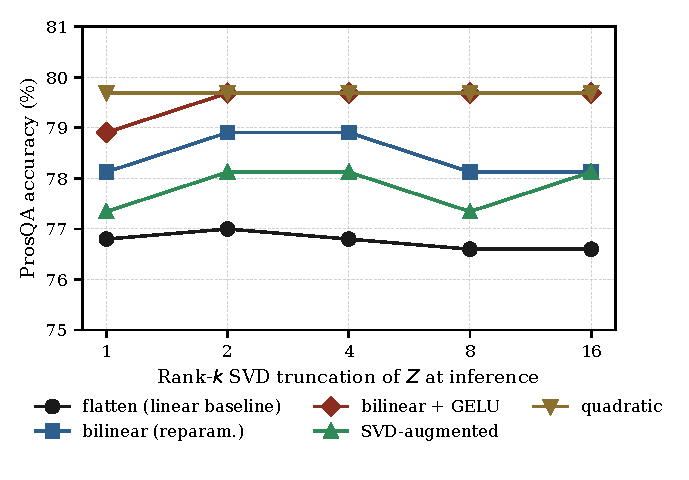
\includegraphics[width=\linewidth]{figures/fig1_rank_curves.pdf}
\caption{Rank-$k$ projection ablation for five readouts on ProsQA.
The flatten (linear) baseline is the Round 3 $\gamma=0$ run. All
four positive-control readouts, including the explicitly
nonlinear-in-$\Z$ Bilinear+GELU, the SVD-augmented readout that
feeds singular values through an MLP, and the quadratic readout
in $\Z\Z^\top$, produce curves flat to within $\sim\!0.8$pp. The
Quadratic readout is perfectly flat at $79.69\%$ across all five
$k$.}
\label{fig:pc}
\end{figure}

\begin{table}[t]
\centering
\small
\setlength{\tabcolsep}{3pt}
\begin{tabular}{lccccccl}
\toprule
Readout & k{=}1 & k{=}2 & k{=}4 & k{=}8 & k{=}16 & $r_s$ & $p$ \\
\midrule
flatten       & 79.0 & 79.0 & 79.0 & 79.0 & 79.0 & $\sim\!0$ & --- \\
bilinear      & 78.1 & 78.9 & 78.9 & 78.1 & 78.1 & $+0.04$ & $0.63$ \\
bilinear+GELU & 78.9 & 79.7 & 79.7 & 79.7 & 79.7 & $-0.13$ & $0.14$ \\
svd-aug       & 77.3 & 78.1 & 78.1 & 77.3 & 78.1 & $+0.02$ & $0.82$ \\
quadratic     & 79.7 & 79.7 & 79.7 & 79.7 & 79.7 & $+0.07$ & $0.46$ \\
\bottomrule
\end{tabular}
\caption{Rank-$k$ ablation accuracies (\%) by readout on $128$
ProsQA test problems. Spearman $r_s$ of per-sample effective rank
against correctness; $p$ is two-sided. No variant's $r_s$ is
statistically significant.}
\label{tab:pc}
\end{table}

All four $p$-values are above $0.14$; the Quadratic readout is
identical across all five $k$. Under the Jacobian hypothesis, the
SVD-augmented readout --- which exposes singular values directly to
the optimizer --- should produce a rank-dependent curve. It does not.

\subsection{Interpretation: a candidate refined mechanism}

The positive control falsifies the narrow reading of
Proposition~\ref{prop:jac} as the \emph{full} explanation of the flat
curves. Readouts with non-constant Jacobians still produce flat
rank-$k$ curves. The mechanism is therefore deeper than readout
linearity alone.

We advance a \emph{candidate refined hypothesis} for future work: the
trained readout's Jacobian at test inputs has an \emph{effectively
rank-1 active subspace in $\Z$}, regardless of whether the readout is
in-principle nonlinear. Concretely: for each trained
positive-control checkpoint, compute
$J(\Z) = \partial\phi/\partial\vecop(\Z)$ at $\Z$ from the test
distribution and report the effective rank of the row-space of $J$
averaged over test examples. The refined hypothesis predicts
$\mathrm{erank}(J) \approx 1$ for Bilinear+GELU, SVD-augmented, and
Quadratic; a value $\geq 4$ would falsify it. This measurement is a
camera-ready experiment we have not yet run on these checkpoints.
We do not claim the refined hypothesis is tested by the current
submission.

Proposition~\ref{prop:jac} remains correct as a sufficient
condition; the positive controls show it is not necessary.

Combined with the three-seed decoupling
(Fig.~\ref{fig:seed-decoupling}), in which the same loss lands at
effective ranks spanning a $3\times$ range across seeds, the natural
conclusion is that the rank of $\Z$ under the matrix-bottleneck
training objective is a free direction in the loss landscape. The
optimizer has no incentive to place it anywhere in particular, and
the readout's local Jacobian shape is not enough to introduce one.

A reviewer might observe that each positive-control readout admits a
\emph{rank-1 output-space shortcut}: the model can route all
task-relevant information through a single singular direction of
$\Z$ (for Quadratic, through $\sigma_1^2 u_1 u_1^\top$) and still
satisfy the loss. This is precisely the claim of the paper --- in
the absence of an objective term that rewards rank, every readout
family we know how to build admits such a shortcut and the optimizer
takes it. The $r_1$ shortcut is available to every readout here;
what distinguishes the positive controls from the flatten baseline
is that their Jacobians are not constant in $\Z$ and yet the
observed curves are identical in shape.

We draw three concrete implications:

\begin{enumerate}
\setlength\itemsep{2pt}
\item \textbf{Rank-$k$ ablation is not a valid probe for
      superposition in matrix-CODI.} A flat rank-$k$ curve does not
      imply the absence of parallel reasoning; it implies that
      whatever the model is doing, it is not using rank as its
      representational axis.
\item \textbf{The fix is at the objective, not the readout.}
      Architectural variants of the readout cannot force the
      objective to reward rank. Candidate fixes (discussed in
      \S\ref{sec:discussion}) are explicit rank rewards, tasks with
      verifiable multi-rank ground truth, or different training
      objectives entirely (e.g.\ step-level supervision as in
      SIM-CoT \citep{shen2025simcot}).
\item \textbf{Nonlinear-in-$\Z$ readouts are not a neutral design
      choice.} The Bilinear+GELU, SVD-augmented, and Quadratic
      readouts each add significant parameter count and constrain
      the readout's Jacobian in a specific way, and none of them
      moved the curve. A designer choosing between them should
      choose on other criteria (speed, gradient stability) and not
      on a presumption of rank expressiveness.
\end{enumerate}

In a matrix-CODI stack, the rank of the matrix thought is \emph{not}
a functional observable, regardless of how the thought is read out;
the matrix-bottleneck training objective does not shape it.

\subsection{Negative control: rank-$k$ ablation on vanilla GPT-2 SFT}
\label{sec:pc-negctrl}

A natural reviewer concern is that the flat rank-$k$ curves in
\S\ref{sec:flat} and \S\ref{sec:pc} are diagnostic of the
matrix-bottleneck objective specifically. We test that by running the
rank-$k$ ablation on a model with \emph{no} matrix bottleneck and
\emph{no} rank-related training: a vanilla GPT-2 small fine-tuned for
ProsQA via standard supervised fine-tuning (\textsc{pure-sft}; no
latent tokens, no $\Z$, no distillation). We trained three seeds
$\{1337, 42, 7\}$ to ${\sim}79$pp ProsQA accuracy (matching the
paper's vanilla baseline), then \emph{constructed} a fake $\Z$ at
inference by reshaping the first $256$ dimensions of the hidden state
$h$ into a $16\!\times\!16$ matrix at the six token positions
immediately preceding the answer-prefix colon (the analog of
matrix-CODI's six latent positions), applied rank-$k$ truncation to
the fake $\Z$ via SVD, and propagated the modified residual through the
remaining transformer blocks. Decoding uses no KV cache so the
intervention re-fires at every step.

\begin{table}[t]
\centering
\small
\setlength{\tabcolsep}{4pt}
\begin{tabular}{lccccc}
\toprule
seed & $k=1$ & $k=2$ & $k=4$ & $k=8$ & $k=16$ \\
\midrule
$1337$ & $79.80$ & $80.20$ & $80.00$ & $80.20$ & $80.00$ \\
$42$   & $79.00$ & $78.80$ & $78.60$ & $78.60$ & $79.00$ \\
$7$    & $78.00$ & $78.00$ & $78.00$ & $78.00$ & $78.20$ \\
\midrule
pooled & $78.93$ & $79.00$ & $78.87$ & $78.93$ & $79.07$ \\
\bottomrule
\end{tabular}
\caption{Negative control: rank-$k$ ablation on vanilla GPT-2 SFT
(no matrix bottleneck, no $\Z$). Fake $\Z$ constructed from
$h[:\!256]$ reshaped to $16\!\times\!16$ at the six analog-latent
positions. Pooled-mean range across $k$ is $0.20$pp. Per-seed Spearman
$r_s$: $+0.32, -0.16, +0.71$ ($n\!=\!500$ test problems each).}
\label{tab:pc-negctrl}
\end{table}

The pooled-mean range across $k$ is $0.20$pp
(Table~\ref{tab:pc-negctrl}). As a sensitivity floor, replacing $h$ at
the same six positions with i.i.d.\ Gaussian noise matched in mean and
standard deviation produces seed accuracies $\{79.6, 79.2, 78.2\}$pp
--- statistically indistinguishable from the unablated $\{80.0, 78.8,
78.0\}$pp. The intervention paradigm is uninformative on this model.

\paragraph{What this implies for the rank-$k$ probe.} The negative
control demonstrates that a flat rank-$k$ curve is consistent with two
substantively different states: (a) a model whose objective is
rank-blind (the paper's main reading), and (b) a model on which the
intervention's chosen positions do not carry functional information,
so any structured perturbation at those positions is invisible.
Vanilla SFT is in case (b) by construction; it has no $\Z$ and no
training to use those positions for reasoning. This means the
rank-$k$ ablation paradigm \emph{cannot, by itself}, distinguish
``loss does not reward rank'' from ``these positions are not where the
task's information flows.''

\paragraph{What it does \emph{not} do to the paper's claim.} The
matrix-CODI model is in a different regime: the bottleneck explicitly
forces information through $\Z$ at those positions during training,
and the trained $\Z$ reaches effective rank $12$--$13$ at $\gamma=0$.
The seed-decoupling result (Fig.~\ref{fig:seed-decoupling}: rank
$\{4,12,13\}$ at matched accuracy) is a model-level property of
matrix-CODI that the negative control does not touch --- a
position-irrelevance reading would not predict that the same loss
lands at $3\!\times\!$ different effective ranks across seeds.
Proposition~\ref{prop:jac} and the four positive-control readouts in
\S\ref{sec:pc} together argue the loss is rank-blind through the
chain rule; the negative control argues the rank-$k$ probe alone is
not enough to test this. Both can be true; we adopt both.

\paragraph{Methodological takeaway.} For any future intervention probe
that claims to measure a structural property of latent representations
(rank, sparsity, activation pattern), the standard practice should be
to run the same intervention on a model that, by construction, does
not have the property. If the probe still produces the diagnostic
shape, the probe is at least partly measuring something other than
the property in question.
